\section{Specification}
% circuit specification
% resource 
% constarint
% sample model : sequence graph
% scheduled equence graph

In pervious section, one of the important specification already be represented in sequencing graph which is the behavioural-level of the circuit model. In this section, the specification will be furthered detailed, including the type and number of resource that will be used in the circuit and the constraints.

At architectural level, resource have their own definition, where it implements different types of function in hardware and can be classified into 3 classes as listed below \cite{main}:

\begin{itemize}
    \item Functional resources : Implementing the arithmetic or logic functions. 
    \item Memory resources : Memory array
    \item Interface resources  : Used to support data transfer including busses and interfacing circuit including external interface for input output
\end{itemize}

Within the scope of this paper, only functional resource will be intensively used. The last specification aspect that will be considered in this paper is constraint. It can be classified into two categories, which are \cite{main}:

\begin{itemize}
    \item Interface constraint : This specification used to ensure that the circuit can be implemented in provided environment like format and timing used in I/O interface.
    \item Implementation constraint : This constraint specified the area constraint, performance constraint and binding constraint.
\end{itemize}

All the constraint are must not specify to give some freedom in synthesizing the architectural model. To narrow the scope of this paper,  the performance constraint will be used including cycle time and latency bound, $\lambda$ that are used to extend the pervious sequencing graph to scheduled sequencing graph as illustrate in ``Fig. \ref{scheduled_sequencing_graph}". Scheduled graph is a function $\varphi : V \xrightarrow{} Z^{+}$, where $\varphi(v_{i})$, denotes the operation start time such that $t_{i} \leq t|_{j} + d_{j}, \forall{i,j}:(v_{j},v_{i}) \in E$ \cite{main}. This graph will be used for further synthesis process.The area constraint entail the number of resource usage, since adding more resource means adding more area to the circuit. All constraint will be further explained in upcoming sections.
 
\begin{figure}[ht]
    \centering
    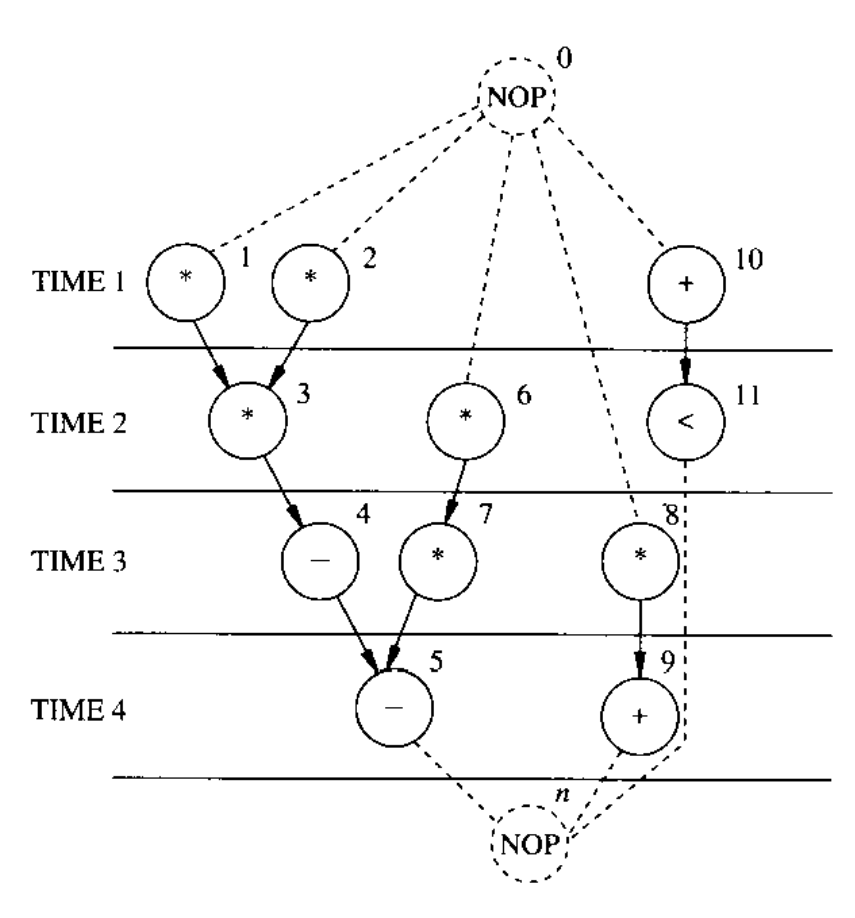
\includegraphics[width=0.5\textwidth]{scheduled_sequencing_graph}
    \caption{scheduled sequencing graph. \cite{main}}
    \label{scheduled_sequencing_graph}
\end{figure}

As shown in `Fig. \ref{scheduled_sequencing_graph}", each vertex represent a type of computation or known as operation type and the resource that execute the operation called resource type. It is also possible that a resource type could execute more than one operation type. ALU, for instance, can do addition, subtraction and comparison. In our circuit model, the resource type that we used is ALU and multiplier as shown in ``Fig. \ref{Example_of_structural_view_at_the_architectural_level}". 

Before going further to the synthesizing process, the stage of the synthesizing process need to be understood. The stages will be discussed in the next section.